% Chapter Template

\chapter{Project Management} % Main chapter title

\label{ChapterX} % Change X to a consecutive number; for referencing this chapter elsewhere, use \ref{ChapterX}

%----------------------------------------------------------------------------------------
%	SECTION 1
%----------------------------------------------------------------------------------------

This chapter highlights the possible ethical issues and risks that could affect the 
development phase of this project. Furthermore, the proposed development methodology and 
project plan are also included in this section.

\section{Risk Management}
To plan out a balanced and well-thought project development schedule, it is essential 
to take into account the inevitable risks that would occur during the phase and therefore, draw out 
efficient risk mitigation strategies to reduce the impact of the risk on the completion 
of this project. Risk Management comprises of four steps:

\begin{itemize}
    \item \textbf{Risk Identification} - Recognizing various risks and labeling their type as follows.\\
    \vspace{-1em}
    \begin{longtable}
        {| p{.12\textwidth} | p{.12\textwidth} | p{.12\textwidth} | p{.15\textwidth} | p{.14\textwidth} | p{.13\textwidth} |} 
        \hline
        Tools & People & Estimation & Requirements & Organization & Technology \\
        \hline
          \end{longtable}
          \vspace{-1em}
    \item \textbf{Risk Analysis} - Analyzing the probability of risk occurance and their impact if it does infact occur. The following color scheme maps the likelihood and impact of a risk.
\\
    \begin{longtable}
        {| p{.12\textwidth} | p{.12\textwidth} | p{.14\textwidth} |} 
        \hline
        \textbf{Color} & \textbf{Likelihood} & \textbf{Impact}  \\
        \hline
        \cellcolor{red} & High & Catastrophic  \\
        \hline
        \cellcolor{yellow} & Medium& Serious  \\
        \hline
        \cellcolor{green} & Low & Tolerable \\
        \hline
          \end{longtable}
        %   \vspace{-1em}
    \item \textbf{Risk Planning} - Devising risk mitigating strategies and thus reduce its impact on the development phase. 
    These strategies could belong to either \textbf{Avoidance}, \textbf{Minimization}, and \textbf{Contingency} categories respectively. 
    \item \textbf{Risk Monitoring} - Regularly assessing each of the possible risks according to its probability of occurrence.
    \end{itemize}

Table \ref{tab:Risk Analysis} summarizes the identified risks and describes possible mitigating strategies.

\begin{longtable}
    {| p{.5\textwidth} | p{.40\textwidth} | p{.40\textwidth}} 
    \hline
    \multicolumn{3}{|c|}{\textbf{Risk Management}}\\
    \hline
    \multicolumn{1}{|c|}{} & \multicolumn{2}{|c|}{\textbf{Planning and Monitoring}}\\
    \hline
    \multicolumn{1}{|c|}{ \parbox[t]{2.5cm}{\textbf{Risk, Type\\Likelihood, \\Impact}}} & \multicolumn{1}{|c|}{\textbf{Monitoring and Avoidance}} & \multicolumn{1}{|c|}{\textbf{Contingency and Minimization}}\\
    \hline
    \multicolumn{1}{|c|}{ \parbox[t]{2.5cm}{\textbf{Insufficient Data}\\Type: Requirements\\\colorbox{yellow}{\textbf{Likelihood}}\\\colorbox{red}{\textbf{Impact}}}} & \multicolumn{1}{|c|}{\parbox[t]{5.75cm}{\textbf{Monitoring:} Review if the learning model underfits on the training data.\\\textbf{Avoidance:} Explore and store all possible open source COVID-19 data sources such as Kaggle.}} & \multicolumn{1}{|c|}{\parbox[t]{5.75cm}{\textbf{Contingency:} Use datasets for other lung diseases and experiment with Transfer Learning.\\ \textbf{Minimization:} Ensure sufficient data from open source COVID-19 repositories are utilized.}}\\\hline
    \multicolumn{1}{|c|}{ \parbox[t]{2.5cm}{\textbf{Inadequate Computation Power}\\Type: Technology\\\colorbox{green}{\textbf{Likelihood}}\\\colorbox{red}{\textbf{Impact}}}} & \multicolumn{1}{|c|}{\parbox[t]{5.75cm}{\textbf{Monitoring:} Track and ensure reasonable time taken for model training.\\\textbf{Avoidance:} Set up GPU powered deep learning libraries such as Tensorflow-GPU before development phase commences, and ensure sufficient storage  on local machine.\vspace{0.3em}}} & \multicolumn{1}{|c|}{\parbox[t]{5.75cm}{\textbf{Contingency:} Utilize GPU powered cloud computing services such as IBM Cloud or MACS computers. \\ \textbf{Minimization:} Ensure GPU powered deep learning libraries are installed and configured on local machine. \vspace{0.2em}}}\\\hline
    \multicolumn{1}{|c|}{ \parbox[t]{2.5cm}{\textbf{Difficulty in Implementation}\\Type: Requirements\\\colorbox{green}{\textbf{Likelihood}}\\\colorbox{red}{\textbf{Impact}}}} & \multicolumn{1}{|c|}{\parbox[t]{5.75cm}{\textbf{Monitoring:} Rank the proposed models based on ease of implementation, model performance and documentation.\\\textbf{Avoidance:} Thorough literature review and research into the proposed models.}} & \multicolumn{1}{|c|}{\parbox[t]{5.75cm}{\textbf{Contingency:} Utilize alternative models which are well documented and are easily usable. \\ \textbf{Minimization:} Allow sufficient time for project development phase after thorough research into existing studies.}}\\\hline
    \multicolumn{1}{|c|}{ \parbox[t]{2.5cm}{\textbf{Loss of Data}\\Type: Tools\\\colorbox{green}{\textbf{Likelihood}}\\\colorbox{red}{\textbf{Impact}}}} & \multicolumn{1}{|c|}{\parbox[t]{5.75cm}{\textbf{Monitoring:} Perform regular checks on backup sources and processes.\\\textbf{Avoidance:} Set up version control and frequently commit changes to the project repository on GitHub.}} & \multicolumn{1}{|c|}{\parbox[t]{5.75cm}{\textbf{Contingency:} Restart project development phase from scratch. \\ \textbf{Minimization:} Ensure that all phases in development are well documented, and utilize it in an unfortunate scenario of data loss.}}\\\hline
    \multicolumn{1}{|c|}{ \parbox[t]{2.5cm}{\textbf{Slow Project Progression}\\Type: Estimation\\\colorbox{yellow}{\textbf{Likelihood}}\\\colorbox{yellow}{\textbf{Impact}}}} & \multicolumn{1}{|c|}{\parbox[t]{5.75cm}{\textbf{Monitoring:} Ensure that the devised project development schedule is followed precisely. \\\textbf{Avoidance:} Ensure all tools and datasets are set up before commencing development phase and start as early as possible.}} & \multicolumn{1}{|c|}{\parbox[t]{5.75cm}{\textbf{Contingency:} Aim to complete the tasks with the highest priority given limited development time. \\ \textbf{Minimization:} Create a rank based priority list for each of the requirements as per project supervisor's recommendation.}}\\\hline
    \multicolumn{1}{|c|}{ \parbox[t]{2.5cm}{\textbf{Personal Health and Deadlines}\\Type: People\\\colorbox{green}{\textbf{Likelihood}}\\\colorbox{yellow}{\textbf{Impact}}}} & \multicolumn{1}{|c|}{\parbox[t]{5.75cm}{\textbf{Monitoring:} Keep track of the deadlines announced and update the project plan accordingly.\\\textbf{Avoidance:} Achieve weekly targets and ensure that the project supervisor is aware of the announced deadlines.}} & \multicolumn{1}{|c|}{\parbox[t]{5.75cm}{\textbf{Contingency:} Complete tasks as per its importance after discussion with project supervisor. \\ \textbf{Minimization:} Adhere to healthy living practices, follow social distancing protocols and keep flexible plans as per new deadlines.}}\\\hline

    \caption{Risk Analysis}
    
      \label{tab:Risk Analysis}
      \end{longtable}

\section{Project Plan}
The various tasks involved in this project and their proposed completion dates for next semester has 
been illustrated using a Gantt Chart which is displayed in Figure \ref{fig:Project Plan}. TeamGantt was used for 
designing the Gantt Chart, Microsoft Planner would be used to keep track of the weekly 
requirements.

\begin{figure}[H]
 \centering
 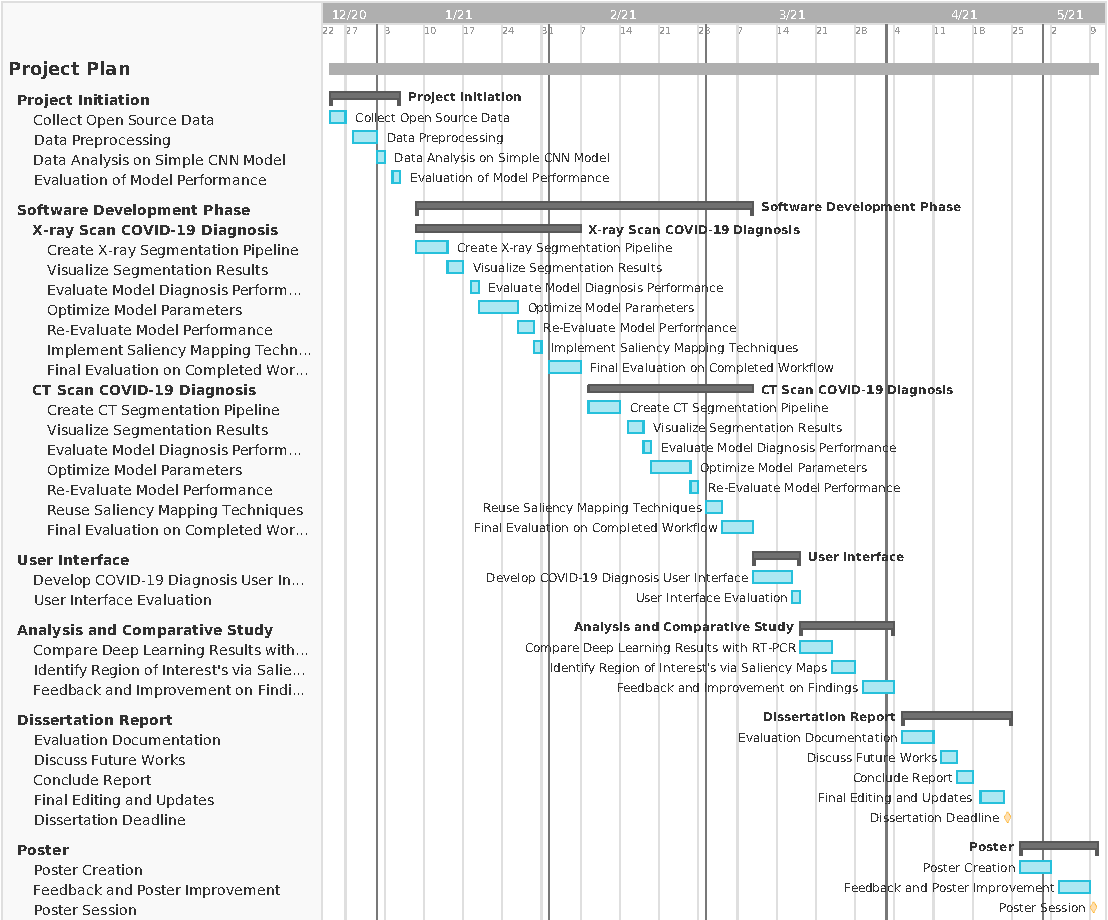
\includegraphics[width=15.5cm]{Images/Project Plan.png}
 \decoRule
 \caption[Project Plan]{Gantt Chart Displaying the proposed Project Plan.}
 \label{fig:Project Plan}
 \end{figure}

\section{Development Methodology}

For this project which involves building a deep learning model 
accompanied by a suitable interface for user interaction, 
an iterative development approach is ideal. \textbf{SCRUM} \cite{SCR}, 
a subset of Agile development methodology proves to be a viable approach. 

Implementing each of the components involved in this project independently 
and adhering to the weekly plan and supervisor's suggestions 
would lead to the deadlines being met and therefore guarantee a successful project completion. 

Further discussion into SCRUM development methodology can be found in Appendix \ref{SCRUM}.

\section{Professional, Legal, Ethical and Social Issues}
\subsection{Professional and Legal Issues}
All research papers discussed in this document are referenced 
accordingly. Any code used from external sources in this project 
shall acknowledge the original authors and would be well documented.
The research papers referenced in this project are either open source 
or have been granted access. The code used for this project shall be 
open source and would be published under the MIT License.

\subsection{Ethical and Social Issues}
No human subjects are involved in this dissertation project. The 
datasets used would be open source and will not 
contain any personal user information and therefore anonymized. Furthermore, all data utilized in this 
project shall be referenced. This project shall not cause any harm to the 
surrounding environment or to any observers.

This project aims to develop a fully automated and rapid COVID-19 diagnosis 
mechanism that reduces virus exposure between patients and 
medical professionals. Through this project, medical professionals 
would receive real-time COVID-19 diagnosis from the provided lung scans, and thus, would be able to rank them based on severity, 
and ultimately save lives.
